\documentclass{standalone}
\usepackage{tikz}
\usetikzlibrary{calc}
\usetikzlibrary{decorations.pathreplacing,calligraphy}
\usepackage{pgfplots}
\usetikzlibrary{intersections, pgfplots.fillbetween}
\usetikzlibrary{snakes}
\usepackage{xcolor}
\usepackage{amsmath}

\begin{document}

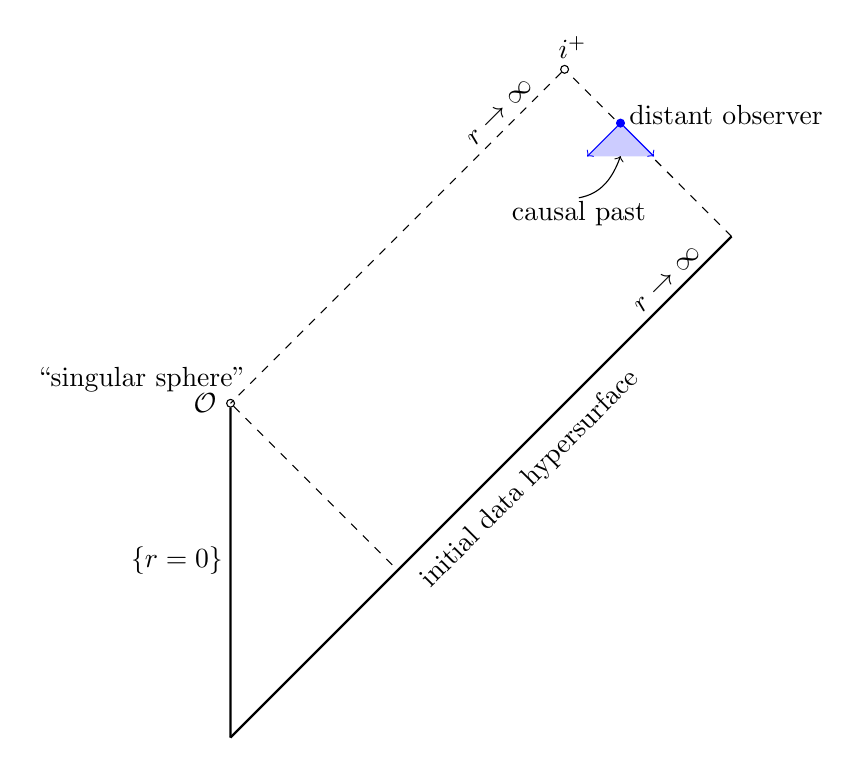
\begin{tikzpicture}[scale=1.5]


\coordinate (n1) at (0,0);
\coordinate (n2) at (45:6);
\draw[thick] (n1) -- (n2);

\coordinate (n3) at ($(n2) + (135:2) $);
\coordinate (b1) at ($(n3) + (-135:2) $);
\node[circle, inner sep = 0, minimum size = .1cm, label = {[xshift=1mm, yshift=-.5mm]above:{$i^+$}}, draw] (node1) at (n3) {};
\draw[dashed] (n2) -- (node1);


\node[label = left:{$\{r=0\}$}] at ($(0,1.5) + (.1,0)$) {};

\coordinate (n8) at ($(node1) + (-135:4)$) ;
\draw[dashed] (node1) --+ (-135:4);

\node[circle, draw, inner sep = 0, minimum size = .1cm, label = left:{$\mathcal{O}$}] (Onode) at (n8) {};

\node[label = left:{``singular sphere"}] (Bnode) at ($(n8)+(0,.2) + (.3,0)$) {};

\draw[thick] (n1) -- (Onode);
\draw[dashed] (Onode) -- ($(Onode) + (-45:2)$);


\coordinate (n7) at (45:4) ;
\node[label = {[rotate = 45]below:{initial data hypersurface}}] at (45:3.4) {};


\coordinate (n95) at ($(0,1.9) + (45:4.67) $ );
\coordinate (n10) at ($(n95) + (-45:.4) $);
\coordinate (n11) at ($(n95) + (-135:.4) $);
\fill[blue!20] ($(0,1.9) + (45:4.67) $ ) -- (n10) -- (n11);
\node[circle, blue, fill, draw, inner sep = 0, minimum size = .1cm, label = {[yshift = 1mm, xshift = -.7mm]right:{distant observer}}] (obs) at (n95) {};

\draw[->, blue] (obs) -- (n10) ;
\draw[->, blue] (obs) -- (n11) ;

\coordinate (n12) at ($(n95) + (0,-.28) $);
\coordinate (n13) at ($(n12) + (-135:.5) $ );

\draw[->] (n13) to[out=10, in = -110] (n12);

\node[label = {[yshift = 2mm]below:{causal past}}] at (n13) {};


\coordinate (b2) at ($(n2) + (-135:.7)  $ ) ;
\coordinate (b3) at ($(n3) + (-135:.7)  $ ) ;
\coordinate (b4) at ($(Onode) + (-45:1)  $ ) ;
\node[label = {[rotate = 45, yshift=-1mm]above:{ $ r\rightarrow \infty $ }}] at (b2) {};
\node[label = {[rotate = 45,yshift=-1mm]above:{ $ r\rightarrow \infty $ }}] at (b3) {};


\end{tikzpicture}

\end{document}